\label {sec:fs-optimization-experiments}
In this section, we describe the preliminary experiments that demonstrate how the choice of a query plan affects the performance. We aim to show that a well-timed switch from an execution graph that is no longer optimal for the current data to a more optimal one would improve performance significantly. First, we present the experiment setup; then, we demonstrate our results. 
% мы хотим показать, что своевременное переключение между планами может улучшить перформанс; мы просто показываем, что разные планы дают разный перформанс, и поэтому переключение между ними дало бы улучшение
\subsection{Setup}

For our experiments, we used the query described in Section \ref{sec:fs-optimization-problem-statement} and the Apache Beam implementation of the NEXMark benchmark model. In this implementation, each entity (\texttt{Person}, \texttt{Auction}, or \texttt{Bid}) is represented via a subclass of the \texttt{Event} class. Each event is generated by an unbounded source in accordance with the provided configuration, which includes parameters such as the arrival rate for each event, the $|Person|:|Auction|:|Bid|$ ratio, the time-based window size, etc. 

First, we execute this query using the plan in which \texttt{Auction} and \texttt{Person} are joined first, and the result is joined with \texttt{Bid}; then, we use the plan in which \texttt{Person} and \texttt{Bid} are joined first (see Section  \ref{sec:fs-optimization-problem-statement}). For each run, we use a different $|Person|:|Auction|:|Bid|$ ratio.

To evaluate performance, we measure latency and throughput for each window. For a join result, we define \textit{latency} as the difference between the maximum arrival time of each of the rows making up the join result and the output time of the resulting row; then, we select the maximum out of the latency values of all the rows in a window. The throughput that we measure is \textit{sustainable throughput}, i.e., the maximum events arrival rate that a streaming system can handle without the continuous buildup of latency.
% sustainable throughput is the maximal rate at which the latency does not start increasing catastrophically
% benchmarking distributed processing systems <-- that is the article from which we use the definition

We have conducted our experiments on a single machine equipped with a 1.4 GHz Intel Core i5-8257U CPU (4 cores) and 8 GB of memory using the Apache Flink runner. Since Flink scales up \cite{karimov2018benchmarking}, we expect that our results for a single worker should scale up to multiple workers.

\subsection{Results}

In the subsequent text the plan which joins \texttt{Auction} and \texttt{Person} first is referred to as \textit{Plan 1}; the plan which joins \texttt{Person} and \texttt{Bid} first is \textit{Plan 2}.
\subsubsection{Latency}

We generated 1000000 events with the arrival rate of 10000 events per second and time-based windows of varying sizes.

Figure \ref{fig:latency_ratio} demonstrates how latency changes depending on data characteristics. The $|Person|:|Auction|:|Bid|$ ratio impacts arrival rate for each kind of entities, thereby influencing latency. As expected, the plan in which \texttt{Person} and \texttt{Auction} are joined first delivers better results when the arrival rate of \texttt{Bid} records significantly overwhelms the rates of \texttt{Person} and \texttt{Auction}, while the plan in which \texttt{Person} and \texttt{Bid} are joined first works best for cases where the rate of \texttt{Auction} records far exceeds those of \texttt{Person} and \texttt{Bid}. 

As Figures \ref{fig:latency_window_5590} and \ref{fig:latency_window_5905} demonstrate, the latency does not grow linearly as the window size increases. This is due to the fact that the join operator processes the records as they arrive instead of starting to process them only after the last record in the window has arrived; thus, the results are ready to emerge shortly thereafter the arrival of the last record in the window.

Figure \ref{fig:latency_diff_against_window_size} demonstrates how the difference in latency for the two execution plans changes with the window size. Since the difference grows as the window size increases, statistics-based optimization should provide an even bigger performance gain for larger windows.

\subsubsection{Throughput}

The parameters for throughput estimation were the same as for the latency estimation. As Figure \ref{fig:throughput_ratio} shows, Plan 2 delivers higher throughput in case of the arrival rate of \texttt{Auction} significantly exceeding that of \texttt{Person} and \texttt{Bid}, while Plan 2 performs better in case of the arrival rate of \texttt{Bid} being significantly higher. This corresponds with the latency measurements. Throughput decreases with the increase of window size, as shown in Figures \ref{fig:throughput_window_5590} and \ref{fig:throughput_window_5905}. Throughput difference does not depend on the window size, Figure \ref{fig:throughput_diff_against_window_size} demonstrates.

\begin{figure*}[t!]
    \begin{subfigure}[b]{0.43\textwidth}
            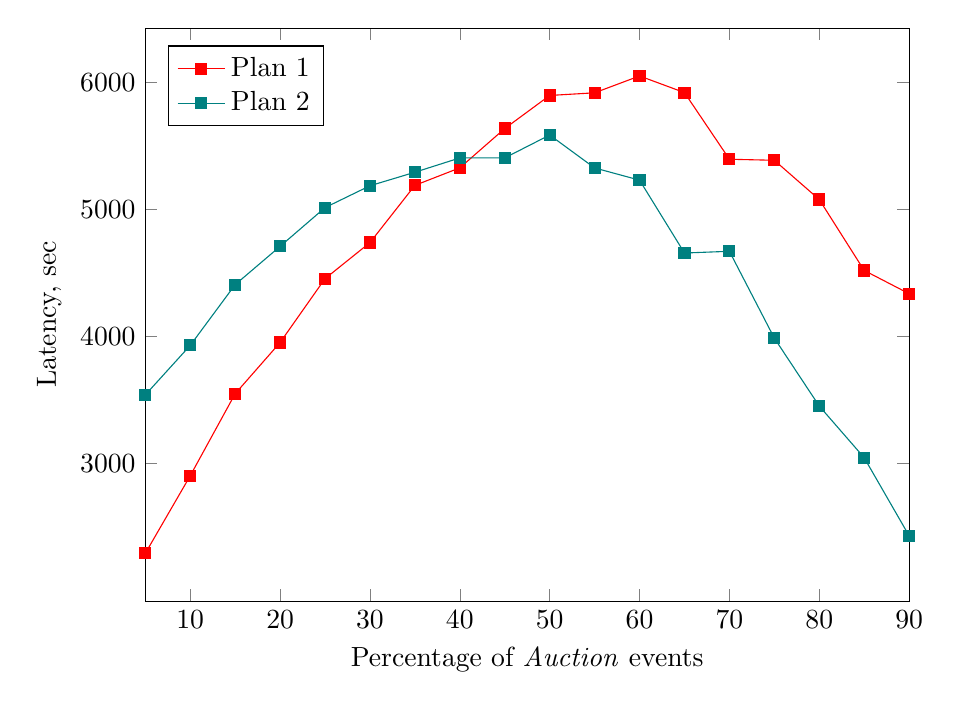
\begin{tikzpicture}
\begin{axis}[
    scale only axis=true,
    width=0.8\textwidth,
    height=0.6\textwidth,
    ytick={3000, 4000, 5000, 6000},
    yticklabels={3000, 4000, 5000, 6000},
    xmin=5, xmax=90,
    legend cell align=left,
    legend pos=north west,
    xlabel={Percentage of \textit{Auction} events},
    ylabel={Latency, sec},
    % x label style={at={(axis description cs:0.5,0.05)},anchor=north},
    % y label style={at={(axis description cs:0.125,0.5)},anchor=center},
]
\addplot[red,mark=square*,mark options={scale=1,solid}] coordinates {
    (5, 2294.73)
    (10, 2905.51)
    (15, 3550.93)
    (20, 3953.99)
    (25, 4456.47)
    (30, 4740.31)
    (35, 5190.68)
    (40, 5328.49)
    (45, 5637.89)
    (50, 5898.18)
    (55, 5918.89)
    (60, 6051.56)
    (65, 5920.56)
    (70, 5396.14)
    (75, 5387.98)
    (80, 5079.04)
    (85, 4520.84)
    (90, 4338.02)
};
\addplot[teal,mark=square*,mark options={scale=1,solid}] coordinates {
    (5, 3541.78)
    (10, 3931.32)
    (15, 4409.38)
    (20, 4710.69)
    (25, 5015.49)
    (30, 5187.45)
    (35, 5293.89)
    (40, 5406.6)
    (45, 5406.6)
    (50, 5586.84)
    (55, 5327.64)
    (60, 5231.65)
    (65, 4658.23)
    (70, 4671.75)
    (75, 3988.29)
    (80, 3453.75)
    (85, 3047.15)
    (90, 2432.85)
};
\legend{
    Plan 1\\
    Plan 2\\
}
\end{axis}
\end{tikzpicture}
            \captionsetup{justification=justified}
            \caption{Latency}
            \label{fig:latency_ratio}
    \end{subfigure}
    \hspace{5mm}
    \begin{subfigure}[b]{0.43\textwidth}
            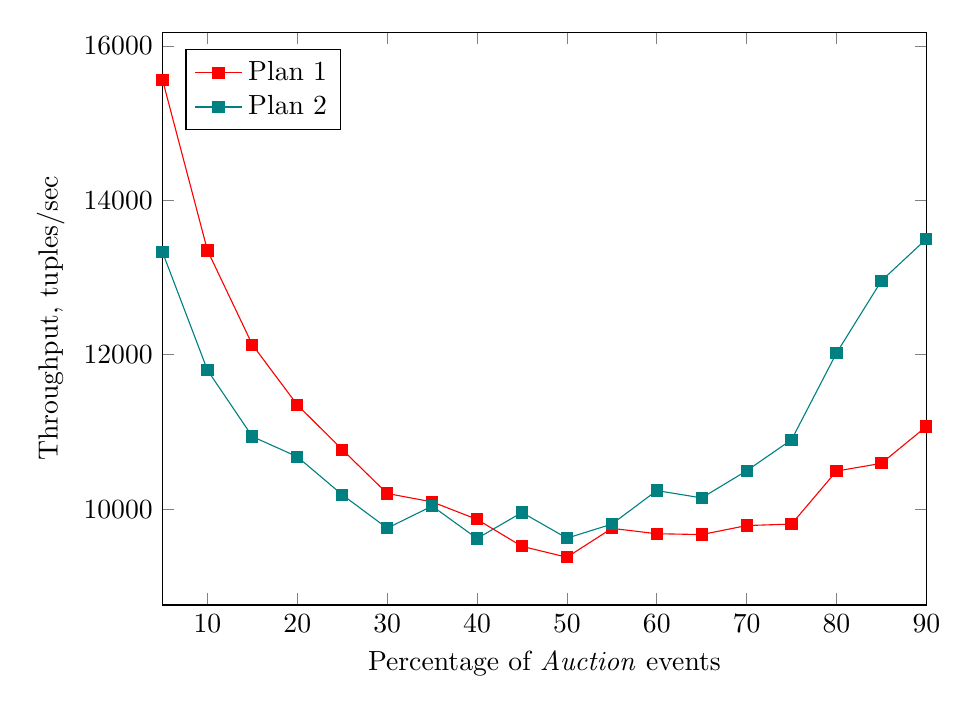
\begin{tikzpicture}
\begin{axis}[
    scale only axis=true,
    width=0.8\textwidth,
    height=0.6\textwidth,
    ytick={10000, 12000, 14000, 16000},
    % yticklabels={3000, 4000, 5000, 6000},
    xmin=5, xmax=90,
    legend cell align=left,
    legend pos=north west,
    xlabel={Percentage of \textit{Auction} events},
    ylabel={Throughput, tuples/sec},
    scaled ticks=false,
     /pgf/number format/.cd,
        use comma,
        1000 sep={}
    % x label style={at={(axis description cs:0.5,0.05)},anchor=north},
    % y label style={at={(axis description cs:0.125,0.5)},anchor=center},
]
\addplot[red,mark=square*,mark options={scale=1,solid}] coordinates {
    (5, 15559.14)
    (10, 13350.6)
    (15, 12128.8)
    (20, 11350.53)
    (25, 10771.7)
    (30, 10203.63)
    (35, 10094.87)
    (40, 9868.2)
    (45, 9519.33)
    (50, 9378.13)
    (55, 9752.17)
    (60, 9682.7)
    (65, 9671.77)
    (70, 9788.26)
    (75, 9807.67)
    (80, 10493.63)
    (85, 10594.13)
    (90, 11070.23)
};
\addplot[teal,mark=square*,mark options={scale=1,solid}] coordinates {
    (5,  13327.4)
    (10, 11800.3)
    (15, 10940.43)
    (20, 10679.2)
    (25, 10187.03)
    (30, 9754.23)
    (35, 10040.93)
    (40, 9621.1)
    (45, 9957.7)
    (50, 9625.23)
    (55, 9806.83)
    (60, 10241.43)
    (65, 10146.33)
    (70, 10497.6)
    (75, 10899.6)
    (80, 12021.9)
    (85, 12957.1)
    (90, 13499.33)
};
\legend{
    Plan 1\\
    Plan 2\\
}
\end{axis}
\end{tikzpicture}
            \captionsetup{justification=justified}
            \caption{Throughput}
            \label{fig:throughput_ratio}
    \end{subfigure}
    \caption{Latency and throughput for different ratios: out of 100 events, $|Person| = 5$, $|Auction|$ is the value on the $x$-axis, $|Bid| = 100 - |Person| - |Auction|$}
    \label{fig:ratio_plots}
\end{figure*}

\begin{figure*}[t!]
    \begin{subfigure}[b]{0.32\textwidth}
            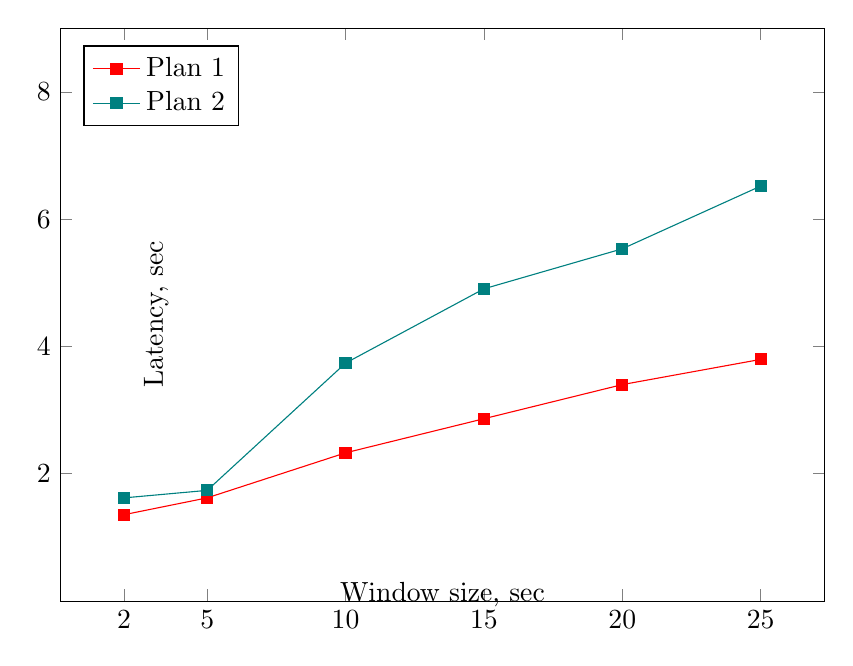
\begin{tikzpicture}
\begin{axis}[
    scale only axis=true,
    width=0.8\textwidth,
    height=0.6\textwidth,
    ymin = 0,
    ymax = 9000,
    ytick={2000, 4000, 6000, 8000},
    yticklabels={2, 4, 6, 8},
    xtick={2, 5, 10, 15, 20, 25},
    xticklabels={$2$, $5$, $10$, $15$, $20$, $25$},
    legend cell align=left,
    legend pos=north west,
    xlabel={Window size, sec},
    ylabel={Latency, sec},
    x label style={at={(axis description cs:0.5,0.05)},anchor=north},
    y label style={at={(axis description cs:0.125,0.5)},anchor=center},
]
\addplot[red,mark=square*,mark options={scale=1,solid}] coordinates {
(2,1357.67)
(5,1621.52)
(10,2328.99)
(15,2864.79)
(20,3400.97)
(25,3796.8)
};
\addplot[teal,mark=square*,mark options={scale=1,solid}] coordinates {
(2,1621.52)
(5,1739.10)
(10,3738.63)
(15,4905.88)
(20,5534.47)
(25,6519.64)
};
\legend{
    Plan 1\\
    Plan 2\\
}
\end{axis}
\end{tikzpicture}
            \captionsetup{justification=justified}
            \caption{$|Person|:|Auction|:|Bid|$ = 5:5:90}
            \label{fig:latency_window_5590}
    \end{subfigure}
    \hspace{2mm}
    \begin{subfigure}[b]{0.32\textwidth}
            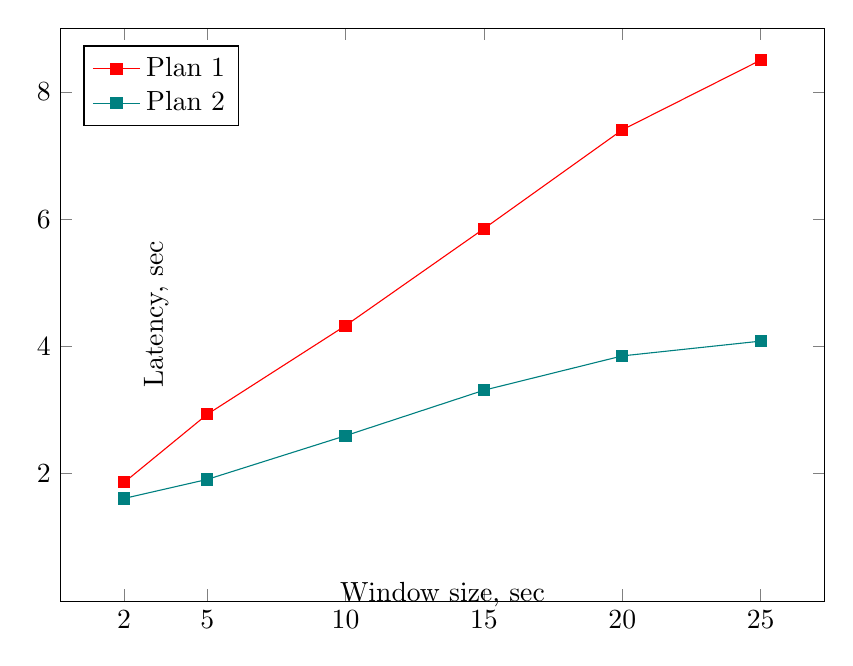
\begin{tikzpicture}
\begin{axis}[
    scale only axis=true,
    width=0.8\textwidth,
    height=0.6\textwidth,
    ymin = 0,
    ymax = 9000,
    ytick={2000, 4000, 6000, 8000},
    yticklabels={2, 4, 6, 8},
    xtick={2, 5, 10, 15, 20, 25},
    xticklabels={$2$, $5$, $10$, $15$, $20$, $25$},
    legend cell align=left,
    legend pos=north west,
    xlabel={Window size, sec},
    ylabel={Latency, sec},
    x label style={at={(axis description cs:0.5,0.05)},anchor=north},
    y label style={at={(axis description cs:0.125,0.5)},anchor=center},
]
\addplot[red, mark=square*, mark options={scale=1,solid}] coordinates {
(2,1864.23)
(5,2933.28)
(10,4327.74)
(15,5850.70)
(20,7403.71)
(25,8498.8)
};
\addplot[teal, mark=square*, mark options={scale=1,solid}] coordinates {
(2,1612.74)
(5,1911.15)
(10,2598.16)
(15,3312.47)
(20,3851.92)
(25,4083.96)
};
\legend{
    Plan 1\\
    Plan 2\\
}
\end{axis}
\end{tikzpicture}
            \captionsetup{justification=justified}
            \caption{$|Person|:|Auction|:|Bid|$ = 5:90:5}
            \label{fig:latency_window_5905}
    \end{subfigure}
    \hspace{2mm}
    \begin{subfigure}[b]{0.32\textwidth}
            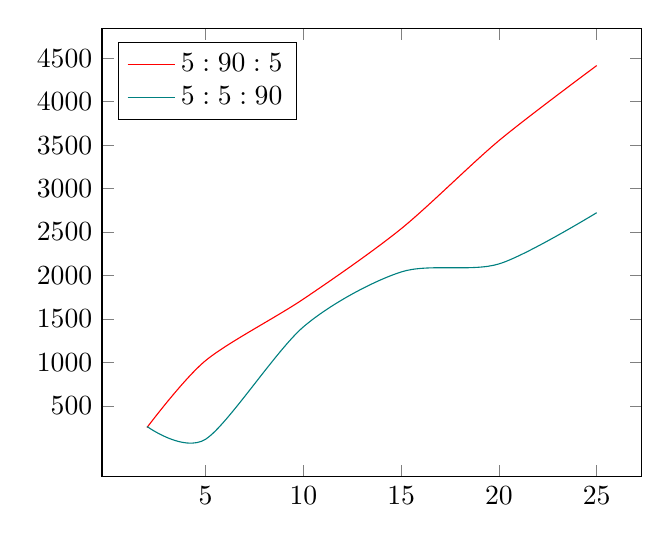
\begin{tikzpicture}
\begin{axis}[
    ytick={500, 1000, 1500, 2000, 2500, 3000, 3500, 4000, 4500},
    yticklabels={$500$, $1000$, $1500$, $2000$, $2500$, $3000$, $3500$, $4000$, $4500$},
    xtick={5, 10, 15, 20, 25},
    xticklabels={$5$, $10$, $15$, $20$, $25$},
    legend cell align=left,
    legend pos=north west
]
\addplot[smooth, red] coordinates {
(2,251.49)
(5,1022.13)
(10,1729.58)
(15,2538.23)
(20,3551.79)
(25,4414.84)
};
\addplot[smooth, teal] coordinates {
(2,263.85)
(5,117.58)
(10,1409.64)
(15,2041.09)
(20,2133.5)
(25,2722.84)
};
\legend{
    $5:90:5$\\
    $5:5:90$\\
}
\end{axis}
\end{tikzpicture}
            \captionsetup{justification=justified}
            \caption{Latency difference for Plans 1 and 2}
            \label{fig:latency_diff_against_window_size}
    \end{subfigure}
    \caption{Latency for different window sizes and $|Person|:|Auction|:|Bid|$ ratios}
    \label{fig:latency_plots}
\end{figure*}

\begin{figure*}[t!]
    \begin{subfigure}[b]{0.32\textwidth}
            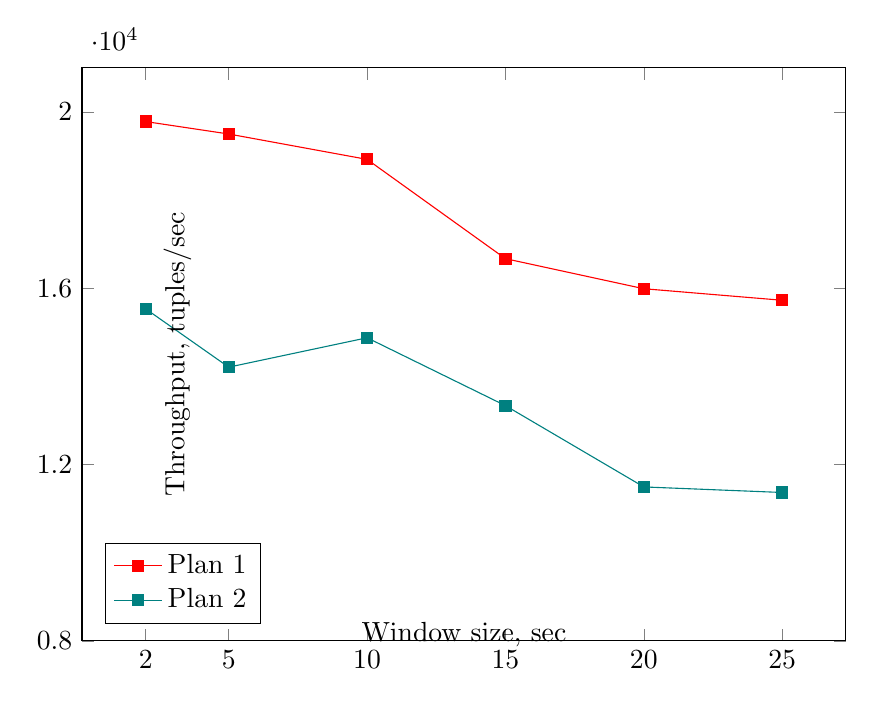
\begin{tikzpicture}
\begin{axis}[
    scale only axis=true,
    width=0.8\textwidth,
    height=0.6\textwidth,
    ymin = 8000,
    ymax = 21000,
    ytick={8000, 12000, 16000, 20000},
    %yticklabels={2, 4, 6, 8},
    xtick={2, 5, 10, 15, 20, 25},
    xticklabels={$2$, $5$, $10$, $15$, $20$, $25$},
    legend cell align=left,
    legend pos=south west,
    xlabel={Window size, sec},
    ylabel={Throughput, tuples/sec},
    x label style={at={(axis description cs:0.5,0.05)},anchor=north},
    y label style={at={(axis description cs:0.125,0.5)},anchor=center},
]
\addplot[red, mark=square*, mark options={scale=1,solid}] coordinates {
(2,19782.8)
(5,19500.8)
(10,18924.7)
(15,16671.4)
(20,15989.5)
(25,15727.7)
};
\addplot[teal, mark=square*, mark options={scale=1,solid}] coordinates {
(2,15532.8)
(5,14209.6)
(10,14876.5)
(15,13336.4)
(20,11491.7)
(25,11365.6)
};
\legend{
    Plan 1\\
    Plan 2\\
}
\end{axis}
\end{tikzpicture}
            \captionsetup{justification=justified}
            \caption{$|Person|:|Auction|:|Bid|$ = 5:5:90}
            \label{fig:throughput_window_5590}
    \end{subfigure}
    \hspace{2mm}
    \begin{subfigure}[b]{0.32\textwidth}
            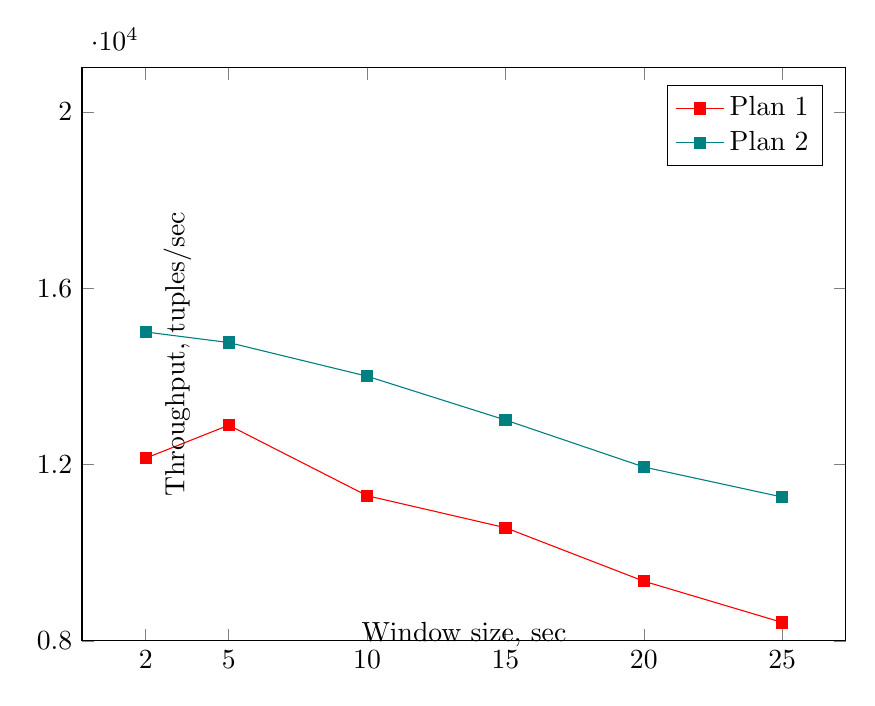
\begin{tikzpicture}
\begin{axis}[
    scale only axis=true,
    width=0.8\textwidth,
    height=0.6\textwidth,
    ymin = 8000,
    ymax = 21000,
    ytick={8000, 12000, 16000, 20000},
    %yticklabels={2, 4, 6, 8},
    xtick={2, 5, 10, 15, 20, 25},
    xticklabels={$2$, $5$, $10$, $15$, $20$, $25$},
    legend cell align=left,
    legend pos=north east,
    xlabel={Window size, sec},
    ylabel={Throughput, tuples/sec},
    x label style={at={(axis description cs:0.5,0.05)},anchor=north},
    y label style={at={(axis description cs:0.125,0.5)},anchor=center},
]
\addplot[red, mark=square*, mark options={scale=1,solid}] coordinates {
(2,12144.02)
(5,12892.16)
(10,11292.62)
(15,10566.26)
(20,9352.6)
(25,8416.64)
};
\addplot[teal, mark=square*, mark options={scale=1,solid}] coordinates {
(2,15007.76)
(5,14768.28)
(10,14004.28)
(15,13010.24)
(20,11943.94)
(25,11262.62)
};
\legend{
    Plan 1\\
    Plan 2\\
}
\end{axis}
\end{tikzpicture}
            \captionsetup{justification=justified}
            \caption{$|Person|:|Auction|:|Bid|$ = 5:90:5}
            \label{fig:throughput_window_5905}
    \end{subfigure}
    \hspace{2mm}
    \begin{subfigure}[b]{0.32\textwidth}
            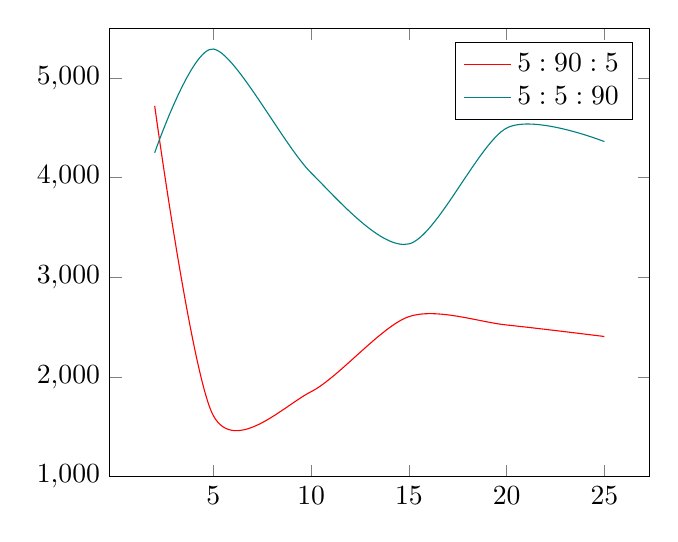
\begin{tikzpicture}
\begin{axis}[
    ymin=1000, ymax=5500,
    xtick={5, 10, 15, 20, 25},
    xticklabels={$5$, $10$, $15$, $20$, $25$},
    legend cell align=left,
    legend pos=north east
]
\addplot[smooth, red] coordinates {
(2,4721.1)
(5,1611.0)
(10,1851.7)
(15,2604.9)
(20,2521.2)
(25,2405.5)
};
\addplot[smooth, teal] coordinates {
(2,4250.0)
(5,5291.2)
(10,4048.2)
(15,3335)
(20,4497.8)
(25,4362.1)
};
\legend{
    $5:90:5$\\
    $5:5:90$\\
}
\end{axis}
\end{tikzpicture}
            \captionsetup{justification=justified}
            \caption{Throughput difference for Plans 1 and 2}
            \label{fig:throughput_diff_against_window_size}
    \end{subfigure}
    \caption{Throughput for different window sizes and $|Person|:|Auction|:|Bid|$ ratios}
    \label{fig:throughput_plots}
\end{figure*}


\subsection{Discussion}

Our experiments demonstrate that streaming query execution performance depends on the plan used for the execution, and the optimality of the plan depends on the data characteristics, which proves the necessity of adaptive optimization of streaming queries. Particularly, the first steps towards adaptive optimization should be predicting statistics for each window and performing runtime graph migration, since the results of the experiments show that even the current planners, such as the Volcano query planner \cite{graefe1993volcano} used in Apache Calcite, which are unaware of whether the data comes from a stream or a table, could use those statistics to produce a better execution plan. These two challenges will be the focus of our future work. After that, the planner can be enhanced by introducing distributed streaming systems-specific operators and their costs.
